\begin{quote}
	\textit{``The major challenge for the future will be effectively and cheaply to shift the sense of presence from one's own body to another, without replacing or excluding the physical world in which we all exist.''}
\end{quote}
\hfill \textit{Waterworth and Waterworth}~\cite{Waterworth2014}
\\
\\
%=========================================================================================================
%=========================================================================================================

\label{introduction}

%=========================================================================================================

A tourist steps into a 15th century chapel. Although the chapel is in remarkable condition for a building that is over 500 years old (it is even still in active use!) it looks markedly different today than it did when it was first built back in 1450. The tourist dons a head-mounted display, which via a pair of front mounted cameras allows her to still see where she is going as she starts to explore the chapel. Once in the centre of the building, she stops walking and presses a button on a controller that she holds in her hand. Her view of the chapel around her disappears and is replaced with an immersive virtual reconstruction of the chapel as it stood over 500 years ago. The view changes appropriately as she turns her head, allowing her to look all around at how the chapel used to be. She releases the button and is returned to the present day, where she continues walking through the chapel until she reaches the altar. She presses the button again and once more her view switches to that of the virtual chapel, which has moved to match her new position at the altar, allowing her to inspect its 1450 counterpart.

This is not an augmented reality system which superimposes virtual objects upon the real world. This is a \textit{parallel reality} system that allows her to switch between seeing the real world and the equivalent vantage in a complete, immersive virtual environment, allowing access to a level of tandem virtuality unprecedented of augmentations.

\afterpage{
\begin{figure}[h]
	\begin{center}
	   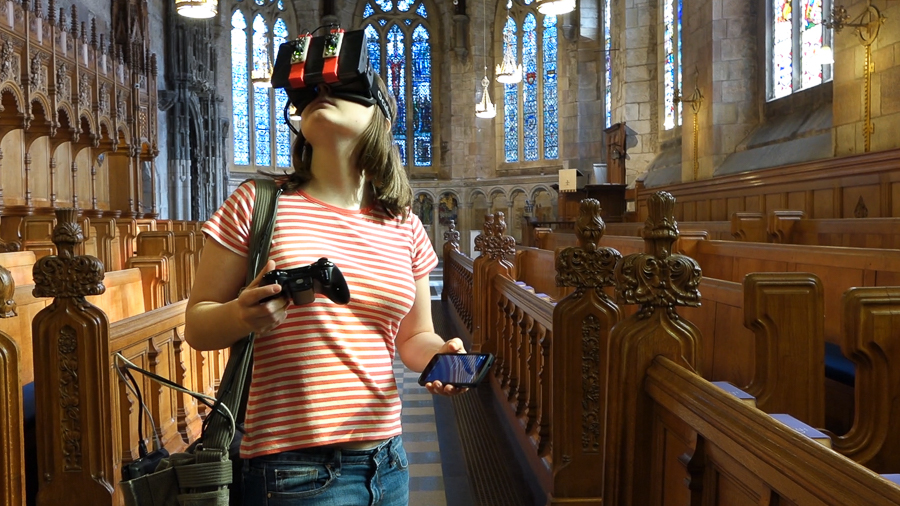
\includegraphics[width=\textwidth]{participant-f-2.jpg}
	\end{center}
	\label{participant-f-2.jpg}
	\caption{The \textit{Mirrorshades} parallel reality platform in use at a 15th century chapel\protect\footnotemark .}
\end{figure}

\footnotetext{ This image is taken from a video that is available to view online at \url{https://www.youtube.com/watch?v=UsDRPjDwr8A}}
}

%=========================================================================================================

\section{Parallel Reality}
\label{intro-parallel-reality}
The central theme of this thesis is the concept of `parallel reality', a new category of alternate reality defined thus:

%\vspace{7mm}

\textbf{Parallel Reality:} A system comprising two environments that the user may freely switch between, one real and the other virtual, both complete unto themselves.

%\vspace{7mm}

%=====================

The concept of alternate realities has become a mainstay both of science fiction and of serious academic research, with the concept of other worlds and how we can either visit them or bring them into our real world keeping authors and scientists alike fascinated for decades. The concept of these `virtual worlds' dates back far into human history, long before mankind's invention of the transistor and the computers that would subsequently harness it.

\begin{quote}
	\textit{``Virtual worlds, or as we will now more broadly define them, immersive experiences delivered through the human imagination, have their origins in deep prehistory. Whether these varieties of nonphysical, dreamlike realities were communicated by our ancestors through the imitation of animals, the incarnation of spirits, the painting of scenes on the stone canvasses of caves, the holding of ceremonial rites in temples, or the elaboration of the human story through the fount of theater, humans have craved and crafted virtual-world experiences from the dawn of artistic and linguistic expression.''}~\cite{Damer2014}
\end{quote}

Within this thesis we are concerned with those alternate realities that through means of computers or other apparatus modify, mediate or create the environmental stimuli received by a subject's senses. Some alternate reality endeavours in this guise have explored the mediation of multiple human senses, from Morton Heilig's 1950's `Sensorama' experience that presented its occupant with a motorcyle ride through combination of film, sound, wind, vibration and odor~\cite{Rheingold1992}, to present day experiences that combine multiple computer generated sensory data such as the Birdly full body flight simulator\footnote{\url{http://birdly.zhdk.ch/}}. However, many are focussed upon visual stimuli alone, with other senses suspended or separated, bracketed into a \textit{``different stream of awareness''}~\cite{Adams2014}.

\begin{quote}
	\textit{``Sight plays such a prominent part in the mental life that the field of vision is sometimes considered almost synonymous with the field of attention.''}~\cite{Lucas1951}
\end{quote}

The 1990s saw a surge of interest around \textit{virtual reality}, promising to immerse users via a head mounted display (HMD) into 3D virtual environments. However with hardware and software simply not advanced enough to meet the hype generated by the news and media, the virtual reality bubble burst and \textit{``the much-hyped `goggles and gloves' virtual reality of the 1990s remains largely unknown in the public domain''}~\cite{Green2014}.

The advent and mass adoption of the smartphone beginning in the early 2000s, with its combination of location sensing (GPS) and orientation sensing (accelerometer and gyroscope) capabilities in a portable package with a screen, camera and Internet access, led to a surge of \textit{augmented reality} applications, which overlaid virtual objects and data upon the view of the real world captured by the phone's rear-facing camera.

The early 2000s also saw the rise of a next generation of persistent multi-user virtual environments, self proclaimed `virtual worlds', with a focus on 3D3C (3D, Community, Creation and Commerce)~\cite{Sevan2008}, including Second Life\footnote{\url{http://secondlife.com/}} from Linden Lab and its open source implementation OpenSim\footnote{\url{http://opensimulator.org/}}. The scientific research potential of these virtual worlds~\cite{Bainbridge2007} led to numerous projects that explored their utility for subjects as diverse as education~\cite{Allison2012}, virtual heritage~\cite{Kennedy2013}, building automation systems\footnote{\url{http://www.ugotrade.com/2007/07/02/eolus-makes-leap-to-3d-internet-on-second-life/}}, data centre visualisation\footnote{\url{http://www-03.ibm.com/press/us/en/pressrelease/23565.wss}} and standards design~\cite{Gelissen2011a}, amongst others.

One such project, led by Joshua Lifton at MIT's Media Lab, introduced \textit{cross reality} as a new category of alternate reality in which the real world and a virtual environment (in this case provided by Second Life) were connected by sensor and actuator infrastructure, allowing bidirectional exchange of media and control information between the two environments, such that actions and events in one could manifest into the other~\cite{Lifton2007a}. This endeavour aimed to mitigate what Lifton identified as the \textit{vacancy problem}, which describes how a person interacting with a virtual environment becomes unaware of their real environment and vice versa, by virtue of not having \textit{``the means to be in more than one place (reality) at a time''}.

The vacancy problem remains an important consideration as we rapidly move into a world where the ubiquity of technology, wireless communications and the explosive popularity of social networking services (SNS) herald the coming of an era in which maintaining a virtual presence (whether 3D or on Facebook) while continuing to function in the real world becomes not just desirable, but the norm, creating instances of \textit{polysocial reality}~\cite{Applin2012} wherever we go.

It is here in the story of alternate realities that this thesis enters. Taking one of the core concepts of cross reality, that of tandem real and virtual environments both complete unto themselves, and extending it to allow the user to engage \textit{visually} with both environments wherever within them they may be, gives rise to parallel reality. With the recent resurgence of interest in HMD based virtual reality, thanks largely to the introduction by Oculus\footnote{\url{https://www.oculus.com/}} of their Rift developer kits that leverage advances in display technology to overcome the shortfalls of the 90s virtual reality fad, and the introduction of novel smartphone based indoor positioning technology from IndoorAtlas\footnote{\url{https://www.indooratlas.com/}}, the \textit{Mirrorshades} parallel reality platform was developed and evaluated as a first foray into this exciting new take on our realities. Where cross reality permitted users an indirect insight into the other environment by means of sensors and actuators, parallel reality grants them the ability to switch between direct visual engagement with each environment - to at one moment view their real surroundings and at the next to view the equivalent vantage in the immersive parallel virtual environment.

%=========================================================================================================

\section{Objectives and Methodology}
\label{objectivesandmethodology}
The design and development of a new alternate reality concept required thorough theoretical comprehension and understanding of existing categories of alternate reality. However to ascertain the merit of a new alternate reality it was all but imperative that it be explored through instantiation, with real world deployment to study users' behaviour, reactions and performance. It is a fundamental tenet of alternate reality experience that somebody actually \textit{have} that experience in order for there to be something to base evaluation upon. While predictions and educated extrapolations can be made about the nature of such an experience through study of the results and observations of previous scenarios that explored existing categories of alternate reality, an involved assessment of a new alternate reality required that it be deployed in the real world and not remain contained to thought experiment or theoretical postulation.

\begin{quote}
	\textit{``There are circumstances where the best or only way to shed light on a proposition, a principle, a material, a process or a function is to attempt to construct something, or to enact something, calculated to explore, embody or test it.''}~\cite{Archer1995}
\end{quote}

%Parallel reality aims to further address the vacancy problem, originally coined by Joshua Lifton, by allowing users to switch freely between equivalent vantage points in two complete environments, one real and the other virtual. While the cross reality systems developed by Lifton succeeded in addressing the `absence' of a person from one environment while participating in the other by introducing changes into one environment based upon triggers in the other, the ability to visually engage with both environments in the true sense of being \textit{``in more than one place (reality) at a time''} was missing from these systems.

The approach taken by this body of research was first to develop a well defined taxonomy of existing alternate reality definitions, in order to correctly situate the new category of parallel reality against them and to inform its design and implementation from the findings and adopted best practices produced by prior alternate reality investigation. This process, which is covered by chapter \ref{chapter-background}, involved effecting updates to several previously established models and creating the combined Milgram/Waterworth model (as explained in section \ref{combined-milgram-waterworth-model}) to sufficiently illustrate and understand the experiential aspect of the proposed parallel reality concept.

The \textit{merit} of the parallel reality concept, however, could not be assessed through such purely theoretical means. While one could have postulated as to the experiential aspects of such a system and how they would manifest during particular tasks and scenarios, it was only through actual creation and application of a parallel reality platform that such postulations could be corroborated or refuted. Thus after the establishment of a strong theoretical foundation of alternate reality taxonomy and experience, an approach of practice-based research, specifically `research through practice'~\cite{Chynoweth2014}, was adopted in order to develop a parallel reality system which could be applied to real world user studies to allow collection and subsequent evaluation of empirical evidence.

Initially the Virtual Time Window platform, discussed in chapter \ref{chapter-vtw}, was developed in order to explore the potential suitability of an existing alternate reality modality of interaction to serve as a platform for investigation into parallel reality experience. When the experiential aspect of the Virtual Time Window did not fully meet with the vision of the parallel reality concept, the Mirrorshades platform, discussed in chapter \ref{chapter-mirrorshades}, was developed in order to fully realise the ideals of the concept via a new modality of alternate reality interaction.

%needs to mention that seated VR is a style of interaction that would be used in the scenario
%and that parallel reality allows exploration of the same content, for the same goal, but in a different manner
The measure of success for the Mirrorshades platform as an instantiation of the parallel reality concept was based upon comparison to a previously established category of alternate reality, by comparing Mirrorshades against a seated virtual reality experience within a virtual heritage scenario. This evaluation is covered by chapter \ref{chapter-eval-1}.

With success of the platform, and the parallel reality concept more generally, strongly indicated by this first user study, two further user studies were undertaken in order to shed light upon how different aspects of the implementation of a parallel reality platform either negatively or positively affected the user experience. These studies, discussed in chapter \ref{chapter-eval-2}, allowed for the construction of a set of best practice recommendations for future parallel reality endeavours.

%=====================

In summary the fundamental research objectives addressed by this thesis were to:

\begin{enumerate}
	\item Introduce the parallel reality concept by situating it within the larger ecosystem of existing categories of alternate reality, through a thorough exploration of existing alternate reality definitions, taxonomies and frameworks, performing updates, modifications and extensions where required.
	
	\item Develop a suitable model for the illustration of experience in parallel reality scenarios, allowing not only for comparison and contrast between parallel reality and other alternate reality experiences, but also for illustration of different implementations of parallel reality experience.
	
	\item Develop a parallel reality system suitable for deployment to real world user studies to effect comparison against previous categories of alternate reality.
	
	%scenario isn't really the word we want - task?
	\item Identify and put into practice suitable assessment techniques to ascertain the merit of parallel reality in relation to previous categories of alternate reality.
	
	\item Identify aspects of the implementation of a parallel reality system that positively or negatively effect the user experience, along with assessment methodologies to ascertain these effects, putting these into practice within real world user studies.

	\item Evaluate user studies to inform creation of best practise recommendations for future parallel reality endeavours.
	
\end{enumerate}

%=========================================================================================================

\section{Collaborations and Publications}
\label{collaborations-and-publications}
While the work presented in this thesis was undertaken principally by myself, it would not have been possible were it not for collaboration. In particular the virtual reconstructions of St Andrews cathedral and St Salvator's chapel, that played a crucial role in the Virtual Time Window and Mirrorshades projects respectively, were created by the members of the Open Virtual Worlds research group working in collaboration with academics from the university's Art History, History and Archaeology departments, as well as with domain experts from heritage organisations including Historic Scotland and the National Trust for Scotland. Particular recognition should go to Sarah Kennedy for her critical role of modelling the reconstructions, Iain Oliver for his systems administration and for providing a Unity\footnote{\url{https://unity3d.com/}} compatible conversion of the OpenSim chapel reconstruction via a tool of his own authoring, and Richard Fawcett with the School of Art History for his invaluable input to these reconstruction processes. Additionally the Unity model of the Jack Cole department building, that played a crucial role in the development and early testing of the Mirrorshades platform, was created by Alex Field.

All other work introduced by this thesis was undertaken by the author.

%=====================

Co-authored peer reviewed papers that cover the process of creation and utilisation of the cathedral and chapel reconstructions (used in chapters \ref{chapter-vtw}, \ref{chapter-mirrorshades}, \ref{chapter-eval-1} and \ref{chapter-eval-2}) include:

\begin{itemize}

	%iED Europe
	\item [1.] Allison, C., Campbell, A., Davies, C., Dow, L., Kennedy, S., Miller, A., Oliver, I. and Perera, I. (2012). Growing the Use of Virtual Worlds in Education: an OpenSim Perspective. Proceedings of the 2nd European Immersive Education Summit.
	
	%AINA
	\item [2.] Oliver, I., Miller, A., Allison, C., Dow, L., Campbell, A., Davies, C., and McCaffery, J. (2013). Towards the 3D Web with Open Simulator. Proceedings of the 27th IEEE International Conference on Advanced Information Networking and Applications.

\end{itemize}

%=====================

In relation to the Virtual Time Window project (see chapter \ref{chapter-vtw}), the following peer reviewed papers were produced:

\begin{itemize}

	%PGNet
	\item [3.] Davies, C., Miller, A., and Allison, C. (2012). Virtual Time Windows: Applying Cross Reality to Cultural Heritage. Proceedings of the 13th Annual Post Graduate Symposium on the Convergence of Telecommunications, Networking and Broadcasting.
	
	%iED Boston
	\item [4.] Davies, C., Allison, C., and Miller, A. (2013). PolySocial Reality for Education: Addressing the Vacancy Problem with Mobile Cross Reality. Proceedings of the 8th Immersive Education Summit.

	%Digital Heritage Marseille
	\item [5.] Davies, C., Miller, A., and Allison, C. (2013). Mobile Cross Reality for Cultural Heritage. Proceedings of the 2013 Digital Heritage International Congress (DigitalHeritage)

\end{itemize}

%=====================

The Cathedral reconstruction that the Virtual Time Window project (see chapter \ref{chapter-vtw}) made use of is covered in greater detail in:

\begin{itemize}

	%iED Europe
	\item [6.] Kennedy, S., Dow, L., Oliver, I., Sweetman, R., Miller, A., Campbell, A., Davies, C., McCaffery, J., Allison, C., Green, D., Luxford, J. and Fawcett, R. (2012). Living history with Open Virtual Worlds: Reconstructing St Andrews Cathedral as a stage for historic narrative. Proceedings of the 2nd European Immersive Education Summit.

\end{itemize}

%=====================

The design and development of the Mirrorshades platform (see chapter \ref{chapter-mirrorshades}) was presented in a poster, with accompanying abstract, and a paper:

\begin{itemize}
	%VRST
	\item [7.] Davies, C., Miller, A., and Allison, C. (2014). A View from the Hill: Where Cross Reality Meets Virtual Worlds.Proceedings of the 20th ACM Symposium on Virtual Reality Software and Technology.

	\item [8.] Davies, C., Miller, A., and Allison, C. (2015). Mobile Onsite Exploration of Parallel Realities with Oculus Rift. Proceedings of the 2015 Digital Heritage International Congress (DigitalHeritage)
	
\end{itemize}

%=====================

Other work from the Open Virtual Worlds group was presented by myself on behalf of the authors:

\begin{itemize}
	
	%iED Boston
	\item [9.] Allison, C., Oliver, I., Miller, A., Davies, C. and McCaffery, J. (2013). From Metaverse to MOOC: Can the Cloud meet Scalability Challenges for Open Virtual Worlds? Proceedings of the 8th Immersive Education Summit.
	
\end{itemize}

%=====================

%=========================================================================================================

\section{Contributions}
\label{intro-contributions}
The contributions of this thesis can be summarized as follows:

\begin{itemize}
	\item The introduction of parallel reality as a new category of alternate reality that allows users to experience complete real and virtual environments in tandem and represents an avenue for further mitigation of the vacancy problem.
	\item The framing of parallel reality through a thorough investigation and extension of previous taxonomies that classify and distinguish between alternate reality terminologies.
	\item The presentation of the combined Milgram/Waterworth model for visualising alternate reality experiences, including those of parallel reality systems.
	\item Exploration into the suitability of an existing state of the art alternate reality modality of interaction (Situated Simulations) for investigation into parallel reality experience, producing the Virtual Time Window platform through extension of the Second Life client.
	\item Development of a new platform for parallel reality, dubbed Mirrorshades, that uses the Unity game engine to combine the modern virtual reality hardware of the Oculus Rift with the novel indoor positioning technology of IndoorAtlas.
	\item Evaluation of the Mirrorshades platform through user studies of a real world use case study within the realm of virtual heritage, including the discussion and application of an established presence questionnaire to a parallel reality experience, both to assess the worth of the concept and to inform future implementations.
	\item Creation and discussion of a set of best practices for future parallel reality endeavours.
\end{itemize}

%=========================================================================================================

\section{Document Overview}

Chapter \ref{chapter-background} surveys the ecosystem of alternate realities, including methods and taxonomies for classifying, categorising and distinguishing between different alternate reality terms, in order to frame the introduction of the parallel reality concept against existing techniques. Chapter \ref{chapter-background} also introduces the combined Milgram/Waterworth model for illustrating parallel reality experience. Chapter \ref{chapter-vtw} describes the development of an initial tablet based parallel reality system, the Virtual Time Window, while chapter \ref{chapter-mirrorshades} details the development of the Mirrorshades HMD based parallel reality platform. Chapters \ref{chapter-eval-1} and \ref{chapter-eval-2} cover the evaluation of the Mirrorshades platform through user studies at a cultural heritage site, the former comparing parallel reality against a more traditional scenario in which virtual reality has already come to be used at such sites and the latter investigating the benefits and drawbacks to different approaches toward parallel reality implementation, resulting in a set of best practice recommendations. Finally chapter \ref{chapter-conclusions} concludes the body of work and postulates on avenues for further investigation into the parallel reality concept.

Table \ref{objectives} provides an overview of the sections of the thesis in which each objective (from section \ref{objectivesandmethodology}) is addressed, along with relevant publications (from section \ref{collaborations-and-publications}).

\vspace{5mm}

\begin{table}[h]
\begin{center}
\begin{minipage}[t]{.6\linewidth}
\begin{center}
\begin{tabularx}{\textwidth}{c *{3}{>{\centering\arraybackslash}X}}
\toprule

\textbf{Objective} & \textbf{Chapter} & \textbf{Related publications} \\

\midrule

1 & \ref{chapter-background} & 3, 4 \& 5 \\

2 & \ref{chapter-background} &  \\

3 & \ref{chapter-vtw} \& \ref{chapter-mirrorshades} & 3, 4, 5 \& 6 \\

4 & \ref{chapter-eval-1} \& \ref{chapter-eval-2} & 7 \& 8 \\

5 & \ref{chapter-eval-1} \& \ref{chapter-eval-2} & 7 \& 8 \\

6 & \ref{chapter-eval-1} \& \ref{chapter-eval-2} & 8 \\

\bottomrule
\end{tabularx}
\caption{Research objectives and corresponding discussion.}
\label{objectives}
\end{center}
\end{minipage}
\end{center}
\end{table}

%=========================================================================================================

%\section{Research Domains}

%\subsection{Virtual Reality}
%including imaging

%\subsection{Virtual Heritage}

%\subsection{Indoor Positioning}

%\subsection{Presence}

%=========================================================================================================

%From William Gibson's `The Gernsback Continuum' and beyond through contemporary cyberpunk literature

%``the reality games of Philip K Dick''~\cite{Sterling1988} and the almost constant virtual overlays of the real world described in Vernor Vinge's Rainbows End~\cite{Vinge2006}



%=====================
%On why alternate realities are predominantly visual?

%\textit{``visual ordination of intellectual knowledge''}

%\textit{``Seeing remains an insistent metaphor for all of cognition only because while the ocular lobes are merely one of our brain's tentacular connections to reality, they are among the most `conscious' of their capacity for information control.''}

%The Mediated Sensorium, Caroline A. Jones




%put into background chapter

%\textit{``virtual reality is a technology that convinces the participant that he or she is actually in another place by substituting the primary sensory input with data received produced by a computer''}~\cite{Heim1998}


%=====================


%can sound alone give us an alternate reality?
%Caroline A. James speaking on the work of Janet Cardiff and George Bures Miller
%\textit{``Cardiff brings segmentation into the present, crafting `sound walks' that layer an alternate reality over the fl\^aneur's perambulations - a fantastic elaboration of the kind of personal soundscape chosen by the iPod user.''}

%=========================================================================================================